\addcontentsline{toc}{chapter}{Занятие 10. Числовые характеристики случайных величин I}
\chapter*{Занятие 10. Числовые характеристики случайных величин I}

\addcontentsline{toc}{section}{Контрольные вопросы и задания}
\section*{Контрольные вопросы и задания}

\subsubsection*{Приведите формулы для вычисления математического ожидания дискретной случайной величины; случайной величины, которая имеет плотность распределения; функции от случайной величины.}

Пусть $ \xi $ --- дискретная случайная величина.
Она может принимать не более чем счётное количество значений.
Принимает значения $x_1, \dotsc, x_n, \dotsc $ с такими вероятностями $p_1, \dotsc, p_n, \dotsc $.
Тогда математическое ожидание вычисляется так
$$M \xi =
\sum \limits_{i=1}^{ \infty } x_i p_i.$$
Для того, чтобы математическое ожидание существовало, необходимо, чтобы ряд сходился адболютно, то есть
$$ \sum \limits_{i=1}^{ \infty } \left| x_i \right| \cdot p_i < + \infty.$$

Пусть $ \xi $ имеет абсолютно непрерывное распределение (имеет плотность распределения $p_{ \xi } \left( x \right) $).
В таком случае математическое ожидание вычисляется ка
$$M \xi =
\int \limits_{- \infty }^{+ \infty } xp_{ \xi } \left( x \right) dx.$$

В случае, если имеем функцию от $ \xi $, математическое ожидание
$$M \varphi \left( x \right) =
\int \limits_{- \infty }^{+ \infty } \varphi \left( x \right) p_{ \xi } \left( x \right) dx.$$

\subsubsection*{Приведите определение дисперсии случайной величины и запишите формулу для её вычисления.}

Дисперсия случайной величины $ \xi $, для которой $ \exists M \xi $,
называется
$$D \xi =
M \left[ \left( \xi - M \xi \right)^2 \right] \leq + \infty.$$
Это мера отклонения случайной величины от своего среднего (математического ожидания).

Для вычисления пользуемся формулой $D \xi = M \xi^2 - \left( M \xi \right)^2.$

\subsubsection*{Сформулируйте свойства математического ожидания и дисперсии.}

Свойства математического ожидания:
\begin{enumerate}
\item если $ \exists M$, то $ \forall c \in \mathbb{R} \, \exists M \left( c \xi \right) $ и $ M \left( c \xi \right) = cM \xi $;
\item если существует $M \xi $ и $M \eta $, то $ \exists M \left( \xi + \eta \right) $ и $M \left( \xi + \eta \right) = M \xi + M \eta $.
Из этих двух условий следует, что математическое ожидание является линейной функцией;
\item $ \exists M \xi \iff \exists M \left| \xi \right| $, и кроме того $ \left| M \xi \right| \leq M \left| \xi \right| $;
\item если $ \xi \geq 0$, то $M \xi \geq 0$;
\item $\xi \geq \eta, \, \exists \xi, \, \exists \eta \Rightarrow M \xi \geq M \eta $;
\item если $ \eta $ и $ \xi $ --- независимые случайные величины,
для которых существует математическое ожидание, то $ \exists M \left( \xi \eta \right) = M \xi \cdot M \eta $.
\end{enumerate}

Свойства дисперсии:
\begin{enumerate}
\item $D \xi \geq 0$'
\item $ \forall \lambda \in \mathbb{R}: \qquad D \left( \lambda \xi \right) = \lambda^2 D \xi $;
\item для независимых $ \eta $ и $ \xi \, D \left( \xi + \eta \right) = D \xi + D \eta $.
\end{enumerate}

\subsubsection*{Запишите неравенство Чебышева.}

Пусть случаайная величина $X: \Omega \rightarrow \mathbb{R}$ определена на вероятностном пространстве
$ \left( \Omega, \mathcal{F}, \mathbb{P} \right) $, а её математическое ожидание $ \mu $ и дисперсия $ \sigma^2$ конечны.
Тогда
$$ \mathbb{P} \left( \left| X - \mu \right| \geq a \right) \leq \frac{ \sigma^2}{a^2},$$
где $a > 0$.

\subsubsection*{Сформулируйте лемму Фату.}

Пусть есть неотрицательная последовательность интегрируемых случайных величин $ \left\{ X_n \right\}_{n=1}^{ \infty }$.
Тогда выполняется следующее неравенство для нижних пределов
$$ \mathbb{E} \left[ \varliminf \limits_{n \to \infty } X_n \right] \leq \varliminf \limits_{n \to \infty } \mathbb{E}X_n.$$

\addcontentsline{toc}{section}{Аудиторные задачи}
\section*{Аудиторные задачи}

\subsubsection*{10.3}

\textit{Задание.}
Случайная величина $ \xi $ имеет дискретное распределение:
$$P \left( \xi = 0 \right) = 0.2,
P \left( \xi = 1 \right) = 0.3,
P \left( \xi = 2 \right) = 0.5.$$
Вычислите: $M \xi, D \xi, M \xi^{10}, M \left( 2 \xi + 1 \right), M \left( \xi - 1 \right)^2$.

\textit{Решение.} Есть дискретная случайная величина, у неё есть 3 значения.
Поэтому $M \xi = 0 \cdot 0.2 + 1 \cdot 0.3 + 2 \cdot 0.5 = 1.3$.

Дисперсия $D \xi = M \xi^2 - \left( M \xi \right)^2$.

Вычислим первое слагаемое $M \xi^2 = 0 \cdot 0.02 + 1 \cdot 0.3 + 4 \cdot 0.5 = 2.3$.

Подставим $D \xi = 2.3 - 1.69 = 0.61$.

Найдём математическое ожидание $M \xi^{10} = 0 \cdot 0.2 + 1 \cdot 0.3 + 1024 \cdot 0.5 = 512.3$.

Воспользуемся линейностью математического ожидания
$$M \left( 2 \xi + 1 \right) =
2 M \xi + 1 =
3.6.$$

Раскроем скобки в следующем выражении
$$M \left( \xi - 1 \right)^2 =
M \xi^2 - 2 M \xi + 1 =
2.3 - 2.6 + 1 =
0.7.$$

\subsubsection*{10.4}

\textit{Задание.} Плотность распределения случайной величины $ \xi $ равна
$$p_{ \xi } \left( x \right) =
\frac{ \lambda }{2} \cdot e^{- \lambda \left| x \right| }, \, \lambda > 0.$$
Вычислите её функцию распредедения, математическое ожидание и дисперсию.

\textit{Решение.} Начнём с математического ожидания
$$M \xi =
\int \limits_{- \infty }^{+ \infty }xp_{ \xi } \left( x \right).$$
Подставляем функцию
$$M \xi =
\int \limits_{- \infty }^{+ \infty } x \cdot \frac{ \lambda }{2} \cdot e^{- \lambda \left| x \right| } dx.$$
Функция нечётная, интегрируется по всей оси, поэтому $M \xi = 0$.

Вычисляем дисперсию.
В данном случае она будет совпадать со вторым моментом
$$D \xi =
M \xi^2 - \left( M \xi \right)^2 =
M \xi^2 =
\int \limits_{- \infty }^{+ \infty } x^2 p_{ \xi } \left( x \right) dx =
\int \limits_{- \infty }^{+ \infty } x^2 \cdot \frac{ \lambda }{2} \cdot e^{- \lambda \left| x \right| } dx.$$
Функция чётная
$$D \xi =
\lambda \int \limits_0^{+ \infty } x^2 e^{- \lambda x} dx.$$
Берём по частям,
$$u = x^2,
dv = e^{- \lambda x} dx,
du = 2xdx,
v = - \frac{1}{ \lambda } \cdot e^{- \lambda x}.$$
Получаем
$$D \xi =
\left. \lambda \cdot x^2 \cdot \left( -1 \right) \cdot \frac{1}{ \lambda } \cdot e^{- \lambda x} \right|_0^{+ \infty } +
\lambda \int \limits_0^{+ \infty } \frac{1}{ \lambda } \cdot e^{- \lambda x} \cdot 2xdx.$$
Ещё раз берём по частям
$$x = u,
dv = e^{- \lambda x}dx,
dx = du,
v = - \frac{1}{ \lambda } \cdot e^{- \lambda x}.$$
Получаем
\begin{equation*}
\begin{split}
D \xi =
\left. 2x \left( - \frac{1}{ \lambda } \cdot e^{- \lambda x} \right) \right|_0^{+ \infty } +
2 \int \frac{1}{ \lambda } \cdot e^{- \lambda x} dx =
\left. - \frac{2}{ \lambda^2} \cdot e^{- \lambda x} \right|_0^{+ \infty } - \\
- \left. \frac{2xe^{- \lambda x}}{ \lambda } \right|_0^{+ \infty } =
\frac{2}{ \lambda^2}.
\end{split}
\end{equation*}

Теперь находим функцию распределения
$$F_{ \xi } \left( x \right) =
\int \limits_{- \infty }^{x} p_{ \xi } \left( y \right) dy =
\begin{cases}
\int \limits_{- \infty }^x \frac{ \lambda }{2} \cdot e^{ \lambda y} dy =
\frac{1}{2} \cdot e^{ \lambda x}, \qquad x < 0, \\
\int \limits_{- \infty }^0 \frac{ \lambda }{2} \cdot e^{ \lambda y} dy + \int \limits_0^x \frac{ \lambda }{2} \cdot e^{- \lambda y} dy = \\
= \left. \frac{1}{2} - \frac{1}{2} \cdot e^{- \lambda y} \right|0-^x =
\frac{1}{2} - \frac{1}{2} \cdot e^{- \lambda x} + \frac{1}{2} = \\
= 1 - \frac{1}{2} \cdot e^{- \lambda x}, \qquad x > 0.
\end{cases}$$

Таким образом,
$$F_{ \xi } \left( x \right) =
\begin{cases}
\frac{1}{2} \cdot e^{ \lambda x}, \qquad x < 0, \\
1 - \frac{1}{2} \cdot e^{- \lambda x}, \qquad x > 0.
\end{cases}$$

\subsubsection*{10.5}

\textit{Задание.} Пусть $ \xi $ --- количество гербов, которые выпали при $n$ подбрасываниях монеты.
Найдите распределение случайной величины $ \xi $.
Вычислите математические ожидания $M \xi, M \xi^2, M \left( 2 \xi + 1 \right) $.

\textit{Решение.} $ \xi = \overline{0, n}$.

Используем биномиальное распределение
$$P \left( \xi = k \right) =
C_n^k \cdot \left( \frac{1}{2} \right)^k \left( 1 - \frac{1}{2} \right)^{n-k} =
C_n^k \left( \frac{1}{2} \right)^n, \,
k = \overline{o, n}.$$

Математическое ожидание
\begin{equation*}
\begin{split}
M \xi =
\sum \limits_{k=0}^n k \cdot P \left( \xi = k \right) =
\sum \limits_{k=0}^n k \cdot C_n^k \cdot \left( \frac{1}{2} \right)^n =
\sum \limits_{k=0}^n \left( \frac{1}{2} \right)^n \cdot k \cdot \frac{n!}{k! \left( n-k \right)!} = \\
= \left( \frac{1}{2} \right)^n \cdot \sum \limits_{k=0}^n \frac{n!}{ \left( k - 1 \right)! \left( n - k \right)!} =
\left( \frac{1}{2} \right)^n \cdot \sum \limits_{k=0}^n \frac{n \left( n-1 \right)!}{ \left( k-1 \right)! \left( n-k \right)!}.
\end{split}
\end{equation*}
Зделаем замену переменных
$$M \xi =
\left( \frac{1}{2} \right)^n \cdot n \cdot \sum \limits_{k=0}^{n-1} C_{n-1}^k =
\left( \frac{1}{2} \right)^n \cdot n \cdot 2^{n-1} =
\frac{n}{2}.$$

Вычислим второй момент
\begin{equation*}
\begin{split}
M \xi^2 =
\sum \limits_{k=0}^n k^2 \cdot P \left( \xi = k \right) =
\sum \limits_{k=0}^n k^2 \cdot C_n^k \cdot \left( \frac{1}{2} \right)^n = \\
= \sum \limits_{k=0}^n \left( \frac{1}{2} \right)^n \cdot k^2 \cdot \frac{n!}{k! \left( n-k \right)!} =
\left( \frac{1}{2} \right)^n \cdot \sum \limits_{k=1}^n \frac{n!k}{ \left( k-1 \right)! \left( n-k \right)!} = \\
= \left( \frac{1}{2} \right)^n \cdot
\left( \sum \limits_{k=1}^n \frac{n!}{ \left( k-2 \right)! \left( n-k \right)!} + \sum \limits_{k=0}^{n-2} \frac{n!}{ \left( k-1 \right)! \left( n-k \right)!} \right) = \\
= \left( \frac{1}{2} \right)^n \left[ n \left( n-2 \right) \cdot \sum \limits_{k=0}^{n-2} C_{n-2}^k + n \sum \limits_{k=0}^{n-2} C_{n-1}^k \right] = \\
= \left( \frac{1}{2} \right)^n \cdot \left[ n \left( n-1 \right) \cdot 2^{n-2} + n \cdot 2^{n-1} \right] =
\frac{n}{4} \left( n-1+2 \right) =
\frac{n \left( n+1 \right) }{2}.
\end{split}
\end{equation*}

Дисперсия
$$D \xi =
M \xi^2 - \left( M \xi \right)^2 =
\frac{n \left( n+1 \right) }{4} - \frac{n^2}{4} =
\frac{n}{4}.$$

Из линейности математического ожидания $M \left( 2 \xi + 1 \right) = 2M \xi + 1 = n + 1$.

\subsubsection*{10.6}

\textit{Задание.} Вычислите:
\begin{enumerate}[label=\alph*)]
\item $M \left| \xi \right| $, если
$$p_{ \xi } \left( x \right) =
\frac{1}{ \sqrt{2 \pi } \sigma } \cdot e^{- \frac{x^2}{2 \sigma^2}};$$
\item $M \sin^2 \pi \xi, Me^{ \xi }$, если
$$p_{ \xi } \left( x \right) =
\begin{cases}
1, \qquad x \in \left[ 0, 1 \right], \\
0, \qquad x \notin \left[ 0, 1 \right];
\end{cases}$$
\item $M \min \left( \left| \xi \right|, 1 \right) $, если
$$p_{ \xi } \left( x \right) =
\frac{1}{ \pi } \cdot \frac{1}{1+x^2}.$$
\end{enumerate}

\textit{Решение.}
\begin{enumerate}[label=\alph*)]
\item Найдём математическое ожидание
$$M \left| \xi \right| =
\int \limits_{- \infty }^{+ \infty } \left| x \right| \cdot \frac{1}{ \sqrt{2 \pi } \sigma } \cdot e^{- \frac{x^2}{2 \sigma^2}}dx.$$
Подинтегральная функция чётная, поэтому
$$M \left| \xi \right| =
2 \int \limits_0^{+ \infty } x \cdot \frac{1}{ \sqrt{2 \pi } \sigma } \cdot e^{- \frac{x^2}{2 \sigma^2}}dx.$$
Введём замену
$$dt = d \left( \frac{x^2}{2 \sigma^2} \right),
t = \frac{x^2}{2 \sigma^2}.$$
Получаем
$$M \left| \xi \right| =
\frac{2 \sigma^2}{ \sqrt{2 \pi } \sigma } \int \limits_0^{+ \infty } e^{-t} dt =
\left. \frac{-2 \sigma }{ \sqrt{2 \pi }} \cdot e^{-t} \right|_0^{+ \infty } =
\frac{2 \sigma }{ \sqrt{2 \pi }};$$
\item это равномерное распределение на отрезке $ \left[ 0, 1 \right] $.

Вычисляем
\begin{equation*}
\begin{split}
M \sin^2 \pi \xi =
\int \limits_{- \infty }^{+ \infty } \sin^2 \pi x \cdot p_{ \xi } \left( x \right) dx =
\int \limits_0^1 \sin^2 \pi x dx =
\int \limits_0^1 \frac{1 - \cos 2x}{2} dx = \\
= \left. \frac{x}{2} \right|_0^1 - \int \limits_0^1 \frac{ \cos 2 \pi x}{2} dx =
\frac{1}{2} - 0 =
\frac{1}{2}.
\end{split}
\end{equation*}

Далее находим
$$Me^{ \xi } =
\int \limits_{- \infty }^{+ \infty } e^x p_{ \xi } \left( x \right) =
\int \limits_0^1 e^x dx =
\left. e^x \right|_0^1 =
e - 1;$$
\item имеем плотность Коши.
Счётного математического ожидания не существует.
Будем вычислять
\begin{equation*}
\begin{split}
M \min \left( \left| \xi \right|, 1 \right) =
\int \limits_{- \infty }^{+ \infty } \min \left( \left| x \right|, 1 \right) p_{ \xi } \left( x \right) dx =
\int \limits_{- \infty }^{-1} \frac{1}{ \pi } \cdot \frac{1}{1+x^2} dx + \\
+ \int \limits_{-1}^1 \left| x \right| p_{ \xi } \left( x \right) dx +
\int \limits_1^{+ \infty } \frac{1}{ \pi } \cdot \frac{1}{1+x^2} dx =
\frac{2}{ \pi } \left( \int \limits_1^{+ \infty } \frac{1}{1+x^2} dx + \int \limits_0^1 \frac{x}{1+x^2} dx \right) = \\
= \frac{2}{ \pi } \left[ \left. arctg x \right|_1^{+ \infty } + \left. \frac{1}{2} \cdot \ln \left( x^2 + 1 \right) \right|_0^1 \right] =
\frac{2}{ \pi } \left( \frac{ \pi }{4} + \frac{1}{2} \cdot \ln 2 \right) =
\frac{1}{2} + \frac{ \ln 2}{ \pi }.
\end{split}
\end{equation*}
\end{enumerate}

\subsubsection*{10.7}

\textit{Задание.} Случайные величины $ \xi $ и $ \eta $ являются независимыми и известно, что $M \xi = 1, M \eta = 2, D \xi = 1, D \eta = 4$.
Вычислите математическое ожидание случайной величины $ \xi^2 + 2 \eta^2 - \xi \eta - 4 \xi + \eta + 4$.

\textit{Решение.} Запишем формулу для дисперсии $D \xi = M \xi^2 - \left( M \xi \right)^2$.

Отсюда выразим второй момент $M \xi^2 = D \xi + \left( M \xi \right)^2$.

Воспользуемся линейностью $M \left( \xi^2 + 2 \eta^2 - \xi \eta - 4 \xi + \eta + 4 \right) = M \xi^2 + \\
+ 2 M \eta^2 - M \xi \cdot M \eta - 4 M \xi + M \eta + 4$.
Переходим к дисперсии.
Это выражение равно $D \xi + \left( M \xi \right)^2 + 2D \eta + 2 \left( M \eta \right)^2 - M \xi \cdot M \eta - 4M \xi + M \eta + 4 = 1 + 1 + 8 + \\
+ 8 - 2 - 4 + 2 + 4 = 18$.

\subsubsection*{10.8}

\textit{Задание.}
Точка P наугад выбрана на границе квадрата ABCD с вершинами в точках $A \left( -1, -1 \right), B \left( -1, 1 \right), C \left( 1, 1 \right) $ и $D \left( 1, -1 \right) $.
Найдите функцию распределения, плотность распределения (если существует), математическое ожидание и дисперсию проекции точки P на:
\begin{enumerate}[label=\alph*)]
\item ось абсцисс;
\item прямую $y = x$.
\end{enumerate}

\textit{Решение.}
\begin{enumerate}[label=\alph*)]
\item Нарисуем квадрат (рис. \ref{fig:108}).

\begin{figure}[h!]
  \centering
  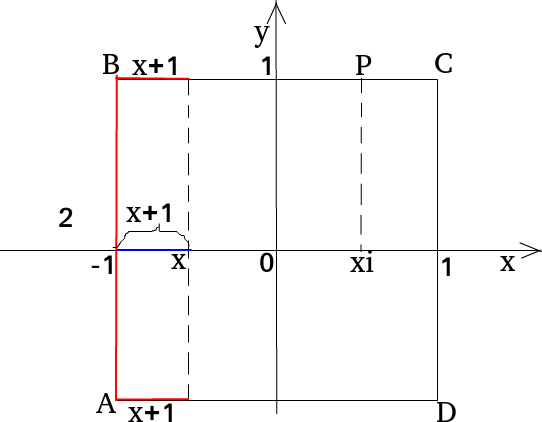
\includegraphics[width=.4\textwidth]{./pictures/10_8.png}
  \caption{Квадрат ABCD}
  \label{fig:108}
\end{figure}

Выберем точку P на границе.
Пусть $ \xi $ --- проекция точки P на ось абсцисс.

Все точки из AB или CD проецируются в одну точку.

Найдём вероятность
$$P \left( \xi = -1 \right) =
P \left( P \in AB \right).$$
AB --- дна из четырёх сторон, поэтому
$$P \left( P \in AB \right) =
\frac{1}{4}.$$

Аналогично
$$P \left( \xi = 1 \right) =
\frac{1}{4}.$$

Берём какое-нибудь $x$.
Для него
$$P \left( \xi \leq x \right) =
\frac{2+2 \left( x+1 \right) }{8} =
\frac{2+x}{4}.$$

Можем записать функцию распределения
$$F \left( x \right) =
\begin{cases}
0, \qquad x < -1, \\
\frac{x+2}{4}, \qquad -1 \leq x \leq 1, \\
1, x \geq 1.
\end{cases}$$

Изобразим её на графике \ref{fig:1081}.

\begin{figure}[h!]
  \centering
  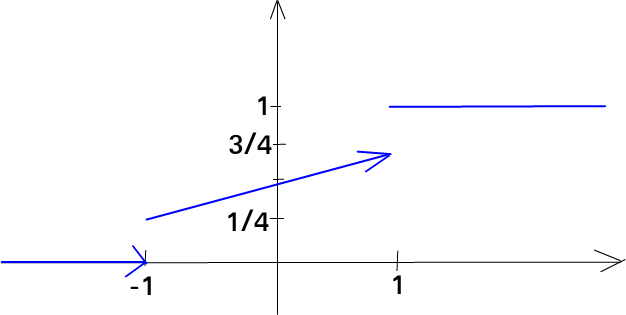
\includegraphics[width=.4\textwidth]{./pictures/10_8_1.png}
  \caption{Функция распределения}
  \label{fig:1081}
\end{figure}

В точке 1 происходит скачек величиной $1/4$ в точку единица.

Случайная величина принимает 2 изолированных значения $-1$ и 1 с вероятностью $1/4$.
На $ \left[ -1, 1 \right) $ она имеет плотность распределения.

Найдём математическое ожидание как интеграл Стилтьеса
$$M \xi =
\int \limits_{- \infty }^{+ \infty } xdF_{ \xi } \left( x \right) =
-1 \cdot \frac{1}{4} + \int \limits_{-1}^1 x \cdot \frac{1}{4} dx + 1 \cdot \frac{1}{4} =
\left. \frac{1}{4} \cdot \frac{x^2}{2} \right|_{-1}^1 =
0.$$

Изменение функции $dF_{ \xi } \left( x \right) $ на $ \left( - \infty, -1 \right) $ и на $ \left[ 1, + \infty \right) $ равно нулю.

Квадрат --- симметрическая фигура относительно точки 0, случайная величина симметрична относительно точки 0.

Дисперсия
\begin{equation*}
\begin{split}
D \xi =
M \xi^2 =
\int \limits_{- \infty }^{+ \infty } x^2 dF_{ \xi } \left( x \right) =
\left( -1 \right)^2 \cdot \frac{1}{4} + \int \limits_{-1}^1 \frac{x^2}{4} dx + \frac{1}{4} =
\left. \frac{1}{2} + \frac{1}{4} \cdot \frac{x^3}{3} \right|_{-1}^1 = \\
= \frac{1}{2} + \frac{1}{4} \left( \frac{1}{3} + \frac{1}{3} \right) =
\frac{1}{2} + \frac{1}{4} \cdot \frac{2}{3} =
\frac{1}{2} + \frac{1}{6} =
\frac{3+1}{6} =
\frac{4}{6} =
\frac{2}{3};
\end{split}
\end{equation*}
\item перерисуем квадрат (рис. \ref{fig:1082}).

\begin{figure}[h!]
  \centering
  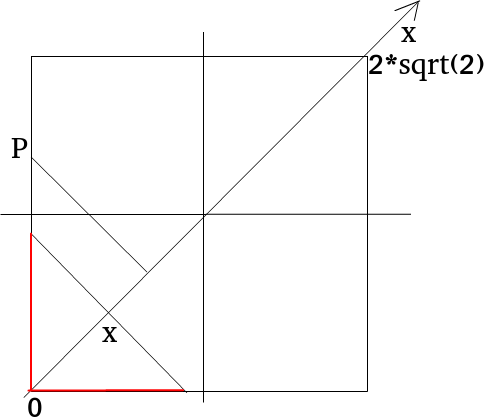
\includegraphics[width=.4\textwidth]{./pictures/10_8_2.png}
  \caption{Квадрат ABCD}
  \label{fig:1082}
\end{figure}

Сделаем замену координат.
Пустим ось $x$ по диагонали.
Выбираем точку на границе, перпендикуляр опускаем на диагональ.
Пусть $ \xi $ --- проекция точки на диагональ.
Считаем вероятность того, что $ \xi \leq x$.

Она равна
$$P \left( \xi \leq x \right) =
2 \cdot \sqrt{2} \cdot x \cdot \frac{1}{8} =
\frac{ \sqrt{2} x}{4} =
\frac{x}{2 \sqrt{2}}.$$

Соответственно если $x < 0$, то это 0, если $x > 2 \sqrt{2} $ --- единица.

Запишем функцию распределения
$$F \left( x \right) =
\begin{cases}
0, \qquad x < 0, \\
\frac{x}{2 \sqrt{2}}, \qquad x \in \left[ 0, 2 \sqrt{2} \right], \\
1, \qquad x > 2 \sqrt{2}.
\end{cases}$$

Отсюда следует, что $ \xi $ имеет равномерное распределение на отрезке $x \in \left[0, 2 \sqrt{2} \right] $.
Математическое ожидание $M \xi = \sqrt{2}$, а дисперсия
$$D \xi = \frac{ \left( 2 \sqrt{2} \right)^2}{12} =
\frac{4 \cdot 2}{12} =
\frac{2}{3}.$$
\end{enumerate}

\subsubsection*{10.9}

\textit{Задание.} Пусть $ \xi $ --- неотрицательная случайная величина с конечным математическим ожидание.
Докажите, что
$$M \xi =
\sum \limits_{i=1}^{ \infty } P \left( \xi \geq 1 \right).$$

\textit{Решение.} $ \xi \geq 0, \xi \in \mathbb{Z}$ --- случайная величина.
По определению
$$M \xi =
\sum \limits_{i=1}^{+ \infty } i \cdot P \left( \xi = i \right) =
\sum \limits_{i=1}^{+ \infty } \left[ iP \left( \xi \geq i \right) - iP \left( \xi \geq i + 1 \right) \right].$$
Обозначим $i + 1 = m$ и разобьём на две суммы
$$M \xi =
\sum \limits_{i=0}^{+ \infty } iP \left( \xi \geq i \right) - \sum \limits_{m=1}^{+ \infty } \left( m-1 \right) P \left( \xi \geq m \right).$$
Обозначим $m=i$, тогда
$$M \xi =
\sum \limits_{i=0}^{+ \infty } iP \left( \xi \geq i \right) - \sum \limits_{i=1}^{+ \infty } \left( i-1 \right) P \left( \xi \geq i \right).$$
Суммируем от единицы
$$M \xi =
\sum \limits_{i=1}^{+ \infty } P \left( \xi \geq i \right)$$

\addcontentsline{toc}{section}{Дополнительные задачи}
\section*{Дополнительные задачи}

\addcontentsline{toc}{section}{Домашнее задание}
\section*{Домашнее задание}

\subsubsection*{10.15}

\textit{Задание.} Случайная величина $ \xi $ имеет дискретное распределение
$$P \left( \xi = 0 \right) = 0.2,
P \left( \xi = 1 \right) = 0.3,
P \left( \xi = 3 \right) = 0.5.$$
Вычислите $M \xi, D \xi, M \xi^5, Me^{ \xi }$.

\textit{Решение.} Есть дискретная случайная величина, которая принимает 3 значения.
Поэтому $M \xi = 0 \cdot 0.2 + 1 \cdot 0.3 + 3 \cdot 0.5 = 0.3 + 1.5 = 1.8$.

По определению $D \xi = M \xi^2 - \left( M \xi \right)^2$.

Найдём второй момент $M \xi^2 = 0 \cdot 0.2 + 1 \cdot 0.3 + 9 \cdot 0.5 = 0.3 + 4.5 = 4.8$.

Тогда дисперсия равна $D \xi = 4.8 - \left( 1.8 \right)^2 = 4.8 - 3.24 = 1.56$.

Найдём математическое ожидание $ \xi^5$.
Это будет $M \xi^5 = 0 \cdot 0.2 + 1 \cdot 0.3 + \\
+ 3^5 \cdot 0.5 = 0.3 + 243 \cdot 0.5 = 0.3 + 121.5 = 121.8$.

Так как экспонента --- непрерывная функция от случайной величины $ \xi $, то $Me^{ \xi } = e^0 \cdot 0.2 + e^1 \cdot 0.3 + e^3 \cdot 0.5 = 0.2 + 0.3 \cdot e + 0.5 \cdot e^3$.

\subsubsection*{10.16}

\textit{Задание.} Игральный кубик подбросили $n$ раз.
Пусть $ \xi $ --- количество выпадений шестёрки.
Найдите распределение $ \xi $, вычислите её математическое ожидание.

\textit{Решение.} $ \xi = \overline{0, n}$.

Найдём вероятность того, что при $n$ подбрасываниях игрального кубика выпало $k$ шестёрок.
Сначала выберем $k$ подбрасываний из $n$, при которых на кубике выпадет шестёрка.
Вероятность того, что выпадет шестёрка равна $1/6$.
Вероятность того, что при $k$ подбрасываниях выпадет шестёрка равна $ \left( 1/6 \right)^k$.
При остальных $n - k$ подбрасываниях может выпасть любая цифра от одного до пяти, а это
$$ \left( 1 - \frac{1}{6} \right)^{n-k} =
\left( \frac{5}{6} \right)^{n-k}.$$
Получаем биномиальное распределение:
$$P \left( \xi = k \right) =
C_n^k \left( \frac{1}{6} \right)^k \left( \frac{5}{6} \right)^{n-k}.$$

Найдём математическое ожидание данной случайной величины
$$M \xi =
\sum \limits_{k=0}^n k \cdot P \left( \xi = k \right) =
\sum \limits_{k=0}^n k \cdot C_n^k \left( \frac{1}{6} \right)^k \left( \frac{5}{6} \right)^{n-k}.$$

Слагаемое при $k = 0$ равно нулю, поэтому суммирование начинаем с единицы
$$M \xi =
\sum \limits_{k=1}^n k \cdot \frac{n!}{k! \left( n-k \right)!} \left( \frac{1}{6} \right)^k \left( \frac{5}{6} \right)^{n-k}.$$

Сократив на $k$, получим
$$M \xi =
\sum \limits_{k=1}^n \frac{n!}{ \left( k-1 \right)! \left( n-k \right)! } \left( \frac{1}{6} \right)^k \left( \frac{5}{6} \right)^{n-k}.$$

В знаменателе прибавим и отнимем единицу
$$M \xi =
\sum \limits_{k=1}^n \frac{n \left( n-1 \right)!}{ \left( k-1 \right)! \left( n - 1 - \left( k-1 \right) \right) } \cdot
\left( \frac{1}{6} \right)^k \left( \frac{5}{6} \right)^{n-k}.$$

Запишем через биномиальный коэффициент
$$M \xi =
\sum \limits_{k=1}^n nC_{n-1}^{k-1} \left( \frac{1}{6} \right)^k \left( \frac{5}{6} \right)^{n-k}.$$

Вынесем $n$ за знак суммы и сделаем замену $k' = k - 1$.
При $k = 1$ получаем, что $k' = 1 - 1 = 0$, при $k = n, k' = n - 1$, при этом $k = k' + 1$.
Тогда
$$M \xi =
n \sum \limits_{k'=0}^{n-1} C_{n-1}^{k'} \left( \frac{1}{6} \right)^{k'+1} \left( \frac{5}{6} \right)^{n-k'-1}.$$

Вынесем $1/6$ за знак суммы
$$M \xi =
\frac{n}{6} \cdot \sum \limits_{k'=0}^{n-1} C_{n-1}^{k'} \left( \frac{1}{6} \right)^{k'} \left( \frac{5}{6} \right)^{n-1-k'}.$$

Получили бином Ньютона
$$M \xi =
\frac{n}{6} \left( \frac{1}{6} + \frac{5}{6} \right)^{n-1} =
\frac{n}{6} \cdot 1^{n-1} =
\frac{n}{6}.$$

\subsubsection*{10.17}

\textit{Задание.} Подброшено $n$ игральных кубиков.
Найдите математическое ожидание суммы и произведения очков.

\textit{Решение.} Найдём математическое ожидание очков, выпавших при одном бросании.
Вероятность выпадения любой из шести граней равна $1/6$.
Имеем дискретную случайную величину $ \xi $, для которой
$$M \xi =
\sum \limits_{k=1}^6 k \cdot \frac{1}{6} =
\frac{1}{6} \cdot \sum \limits_{k=1}^6 k =
\frac{1}{6} \cdot 21 =
\frac{7}{2}.$$

Из свойств математического ожидания, если существуют $M \xi $ и $M \eta $, то существует $M \left( \xi + \eta \right) $ и $M \left( \xi + \eta \right) = M \xi + M \eta $.
Следовательно математическое ожидание суммы очков, выпавших при $n$ подбрасываниях игрального кубика, равно
$$M \xi_1 =
n \cdot \frac{7}{2} =
\frac{7n}{2}.$$

Из свойств математического ожидания,
если случайные величины $ \xi $ и $ \eta $ независимы,
$M \xi $ и $M \eta $ существуют, то $M \left( \xi \eta \right) $ существует и $M \left( \xi \eta \right) = M \xi \cdot M \eta $.

Так как подбрасывания кубика независимы, воспользуемся этим свойством
$$M \xi_2 =
\left( \frac{7}{2} \right)^n.$$

\subsubsection*{10.18}

\textit{Задание.} Пусть $ \xi $ имеем плотность распределения
$$p \left( x \right) =
\frac{1}{ \sqrt{2 \pi } \sigma } \cdot e^{- \frac{ \left( x-a \right)^2}{2 \sigma^2}}$$
(нормальное распределение с параметрами $ \left( a, \sigma^2 \right) $).
Вычислите $ M \left| \xi - a \right| $.

\textit{Решение.} По определению математического ожидания случайной величины, для которой задана плотность распределения
$$M \left| \xi - a \right| =
\int \limits_{- \infty }^{+ \infty } \left| x - a \right| \cdot \frac{1}{ \sqrt{2 \pi } \sigma } \cdot e^{- \frac{ \left( x - a \right)^2}{2 \sigma^2}} dx.$$

Подинтегральная функция чётная, поэтому
$$M \left| \xi - a \right| =
2 \int \limits_0^{+ \infty } \left( x - a \right) \cdot \frac{1}{ \sqrt{2 \pi } \sigma } \cdot e^{- \frac{ \left( x - a \right)^2}{2 \sigma^2}} dx.$$

Введём замену
$$t = \frac{ \left( x-a \right)^2}{2 \sigma^2},
dt = d \left( \frac{ \left( x-a \right)^2}{2 \sigma^2} \right) = \frac{2 \left( x-a \right) }{2 \sigma^2} dx = \frac{x-a}{ \sigma^2} dx,$$
откуда
$$dx = \frac{ \sigma^2 dt}{x-a}.$$
Подставим введённую замену в выражение
\begin{equation*}
\begin{split}
M \left| \xi - a \right| =
2 \int \limits_0^{+ \infty } \left( x-a \right) \cdot \frac{1}{ \sqrt{2 \pi } \sigma } \cdot e^{-t} \cdot \frac{ \sigma^2}{x-a} dt =
2 \int \limits_0^{+ \infty } \frac{1}{ \sqrt{2 \pi }} \cdot \sigma e^{-t} dt = \\
= \frac{2}{ \sqrt{2 \pi }} \cdot \sigma \int \limits_0^{+ \infty } e^{-t} dt =
\left. - \sqrt{ \frac{2}{ \pi }} \cdot \sigma e^{-t} \right|_0^{+ \infty } =
- \sqrt{ \frac{2}{ \pi }} \cdot \sigma \cdot \left( e^{- \infty } - e^0 \right) = \\
= - \sqrt{ \frac{2}{ \pi }} \cdot \sigma \left( 0 - 1 \right) =
\sqrt{ \frac{2}{ \pi }} \cdot \sigma.
\end{split}
\end{equation*}

\subsubsection*{10.19}

\textit{Задание.} Случайная величина $ \xi $ имеет плотность распределения
$$p \left( x \right) =
\begin{cases}
\frac{ \sin x}{2}, \qquad x \in \left[ 0, \pi \right], \\
0, \qquad x \notin \left[ 0, \pi \right].
\end{cases}$$
Вычислите:
$$P \left( \xi \in \left[ \frac{ \pi }{4}, \frac{ \pi }{3} \right] \right);
M \xi;
M \cos \xi.$$

\textit{Решение.} Найдём вероятность того, что $ \xi $ попадёт в указанный отрезок
\begin{equation*}
\begin{split}
P \left( \xi \in \left[ \frac{ \pi }{4}, \frac{ \pi }{3} \right] \right) =
\int \limits_{ \frac{ \pi }{4}}^{ \frac{ \pi }{3}} p_{ \xi } \left( x \right) dx =
\int \limits_{ \frac{ \pi }{4}}^{ \frac{ \pi }{3}} \frac{ \sin x}{2} dx =
\frac{1}{2} \cdot \int \limits_{ \frac{ \pi }{4}}^{ \frac{ \pi }{3}} \sin x dx =
\left. - \frac{1}{2} \cdot \cos x \right|_{ \frac{ \pi }{4}}^{ \frac{ \pi }{3}} = \\
= - \frac{1}{2} \cdot \left( \cos \frac{ \pi }{3} - \cos \frac{ \pi }{4} \right) =
- \frac{1}{2} \left( \frac{1}{2} - \frac{ \sqrt{2}}{2} \right) =
\frac{1}{2} \cdot \frac{ \sqrt{2} - 1}{2} =
\frac{ \sqrt{2} - 1}{4}.
\end{split}
\end{equation*}

Найдём математическое ожидание
$$M \xi =
\int \limits_{- \infty }^{+ \infty } xp_{ \xi } \left( x \right) dx =
\int \limits_0^{ \pi } x \cdot \frac{ \sin x}{2} dx.$$

Вынесем $1/2$ за знак интеграла
$$M \xi =
\frac{1}{2} \int \limits_0^{ \pi } x \sin x dx.$$

Берём интеграл по частям
$$u = x,
dv = \sin x dx,
du = dx,
v = \int \sin x dx = - \cos x.$$
Подставляем
$$M \xi =
\left. - \frac{1}{2} \cdot x \cos x \right|_0^{ \pi } + \frac{1}{2} \int \limits_0^{ \pi } \cos x dx =
\left. - \frac{1}{2} \cdot \pi \cos \pi + \frac{1}{2} \sin x \right|_0^{ \pi } =
\frac{- \pi \left( -1 \right) }{2} =
\frac{ \pi }{2}.$$

Найдём математическое ожидание косинуса
$$M \cos \xi =
\int \limits_{- \infty }^{+ \infty } \cos x \cdot p_{ \xi } \left( x \right) dx =
\int \limits_0^{ \pi } \cos x \cdot \frac{ \sin x}{2} dx.$$

Вынесем $1/2$ за знак интеграла
$$M \cos \xi =
\frac{1}{2} \int \limits_0^{ \pi } \sin x \cdot \cos x dx.$$

Умножим и поделим на 2
$$M \cos \xi =
\frac{1}{4} \int \limits_0^{ \pi } \sin \left( 2x \right) dx.$$

Сделаем замену
$$2x = y,
dy = 2dx,
dx = \frac{dy}{2}.$$
Получим
\begin{equation*}
\begin{split}
M \cos \xi =
\frac{1}{4} \int \limits_0^{2 \pi } \sin y \cdot \frac{dy}{2} =
\frac{1}{8} \int \limits_0^{2 \pi } \sin y dy =
\left. - \frac{1}{8} \cdot \cos y \right|_0^{2 \pi} = \\
= - \frac{1}{8} \left( \cos \left( 2 \pi \right) - \cos 0 \right) =
- \frac{1}{8} \left( 1 - 1 \right) =
0.
\end{split}
\end{equation*}

\subsubsection*{10.20}

\textit{Задание.} Случайные величины $ \xi $ и $ \eta $ являются независимыми и известно, что $M \xi = 1, M \eta = 2, D \xi = 1, D \eta = 4$.
Вычислите:
\begin{enumerate}[label=\alph*)]
\item $M \left( \xi + \eta + 1 \right)^2$;
\item $D \xi \eta $.
\end{enumerate}

\textit{Решение.} Запишем формулу для дисперсии $D \xi = M \xi^2 - \left( M \xi \right)^2$.

Отсюда выразим второй момент $M \xi^2 = D \xi + \left( M \xi \right)^2 = 1 + 1 = 2$.

Аналогичные действия проделываем для $ \eta $ и получаем
$$M \eta^2 =
D \eta + \left( M \eta \right)^2 =
4 + 4 =
8.$$

\begin{enumerate}[label=\alph*)]
\item Найдём $M \left( \xi + \eta + 1 \right)^2$.
Раскроем скобки
\begin{equation*}
\begin{split}
M \left( \xi + \eta + 1 \right)^2 =
M \left[ \left( \xi + \eta \right)^2 + 2 \left( \xi + \eta \right) + 1 \right] = \\
= M \left( \xi^2 + 2 \xi \eta + \eta^2 + 2 \xi + 2 \eta + 1 \right).
\end{split}
\end{equation*}

Пользуемся линейностью
$$M \left( \xi + \eta + 1 \right)^2 =
M \xi^2 + 2 M \xi M \eta + M \eta^2 + 2M \xi + 2M \eta + 1.$$

Подставим числовые значения $M \left( \xi + \eta + 1 \right)^2 = 2 + 2 \cdot 1 \cdot 2 + 8 + 2 \cdot 1 + \\
+ 2 \cdot 2 + 1 = 2 + 4 + 8 + 2 + 4 + 1 = 21$;
\item по определению $D \xi \eta = M \left( \xi \eta \right)^2 - \left[ M \left( \xi \eta \right) \right]^2$.

Так как случайные величины независимы, то
$$D \left( \xi \eta \right) =
M \left( \xi^2 \cdot \eta^2 \right) - \left( M \xi \cdot M \eta \right)^2 =
M \xi^2 \cdot M \eta^2 - \left( M \xi \right)^2 \left( M \eta \right)^2.$$

Подставим числовые значения $D \left( \xi \eta \right) = 2 \cdot 8 - 1 \cdot 4 = 16 - 4 = 12$.
\end{enumerate}
